\section{Vision Transformer (ViT)}
\begin{figure}[]
    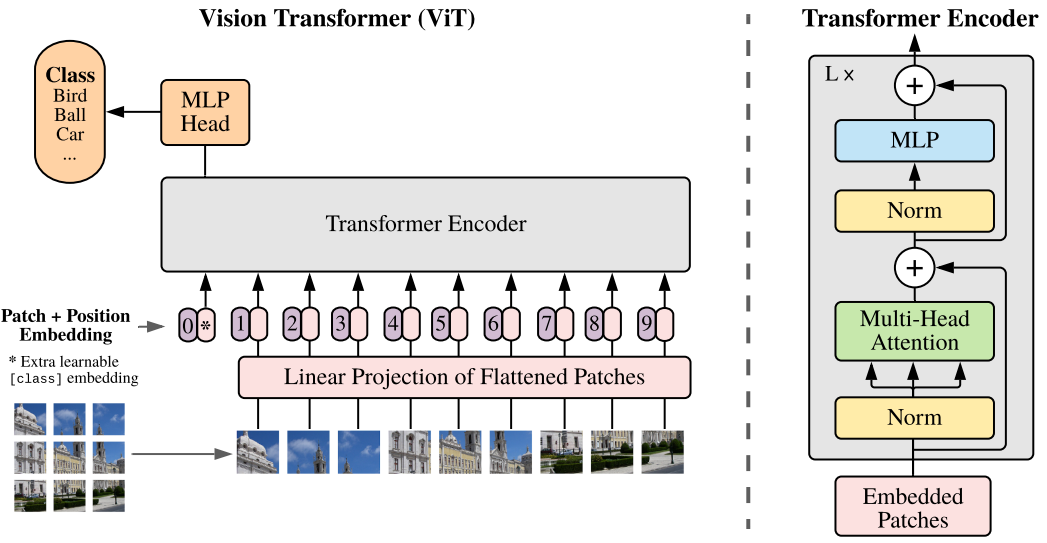
\includegraphics[width=\columnwidth]{figures/VisionTransformer/ViT.png}
\end{figure}
\begin{itemize}
    \item Extract square Images Patches
    \item Flatten Patches and project them to the embedding dimension D
    \item These embeddings are input to the Transformer
    \item Output of Transformer is fed into MLP or a singel layer
    \item Position embeddings added to input embeddings
\end{itemize}

Excellent results when pretrained on larger dataset(14M-300M)images and fine-tuned.

\subsection{Vertical Design}
\begin{figure}[!h]
    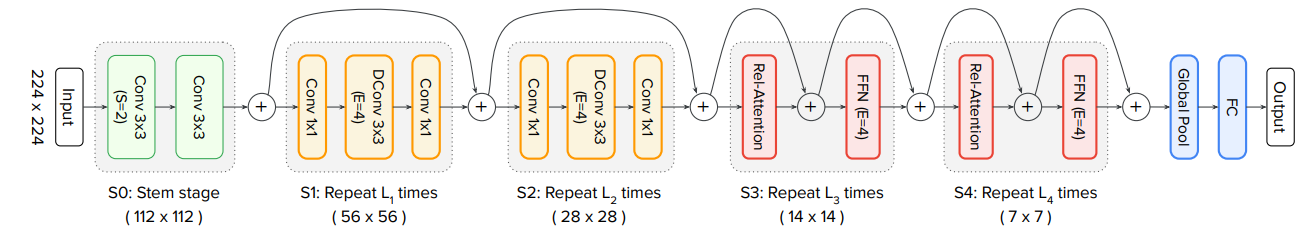
\includegraphics[width=\columnwidth]{figures/VisionTransformer/verticalDesign.png}
\end{figure}
\begin{itemize}
    \item Applying the relative-attention at pixel level is Computationally not possible
    \item A down-sampling of the image is needed
    \item Mimics CNNs architecture
\end{itemize}
\subsection{Relative self-Attention}
\begin{itemize}
    \item Considers realitve position of tokens
    \item  
\end{itemize}